% Appendix: full qualitative stacks + LoRA failure cases
\appendix
\section{Supplementary Qualitative Results}
\label{sec:appendix_qual}

The main paper (Fig.~\ref{fig:task1},~\ref{fig:task2}) shows representative single-case examples. Below we provide the full six-sample qualitative stacks (Figs.~\ref{fig:app_seg_stack}--\ref{fig:app_age_stack}) and document common LoRA failure modes (Figs.~\ref{fig:app_seg_failure}--\ref{fig:app_age_failure}).

\subsection{Full Six-Sample Stacks (High Performers)}

\begin{figure}[t]
\centering
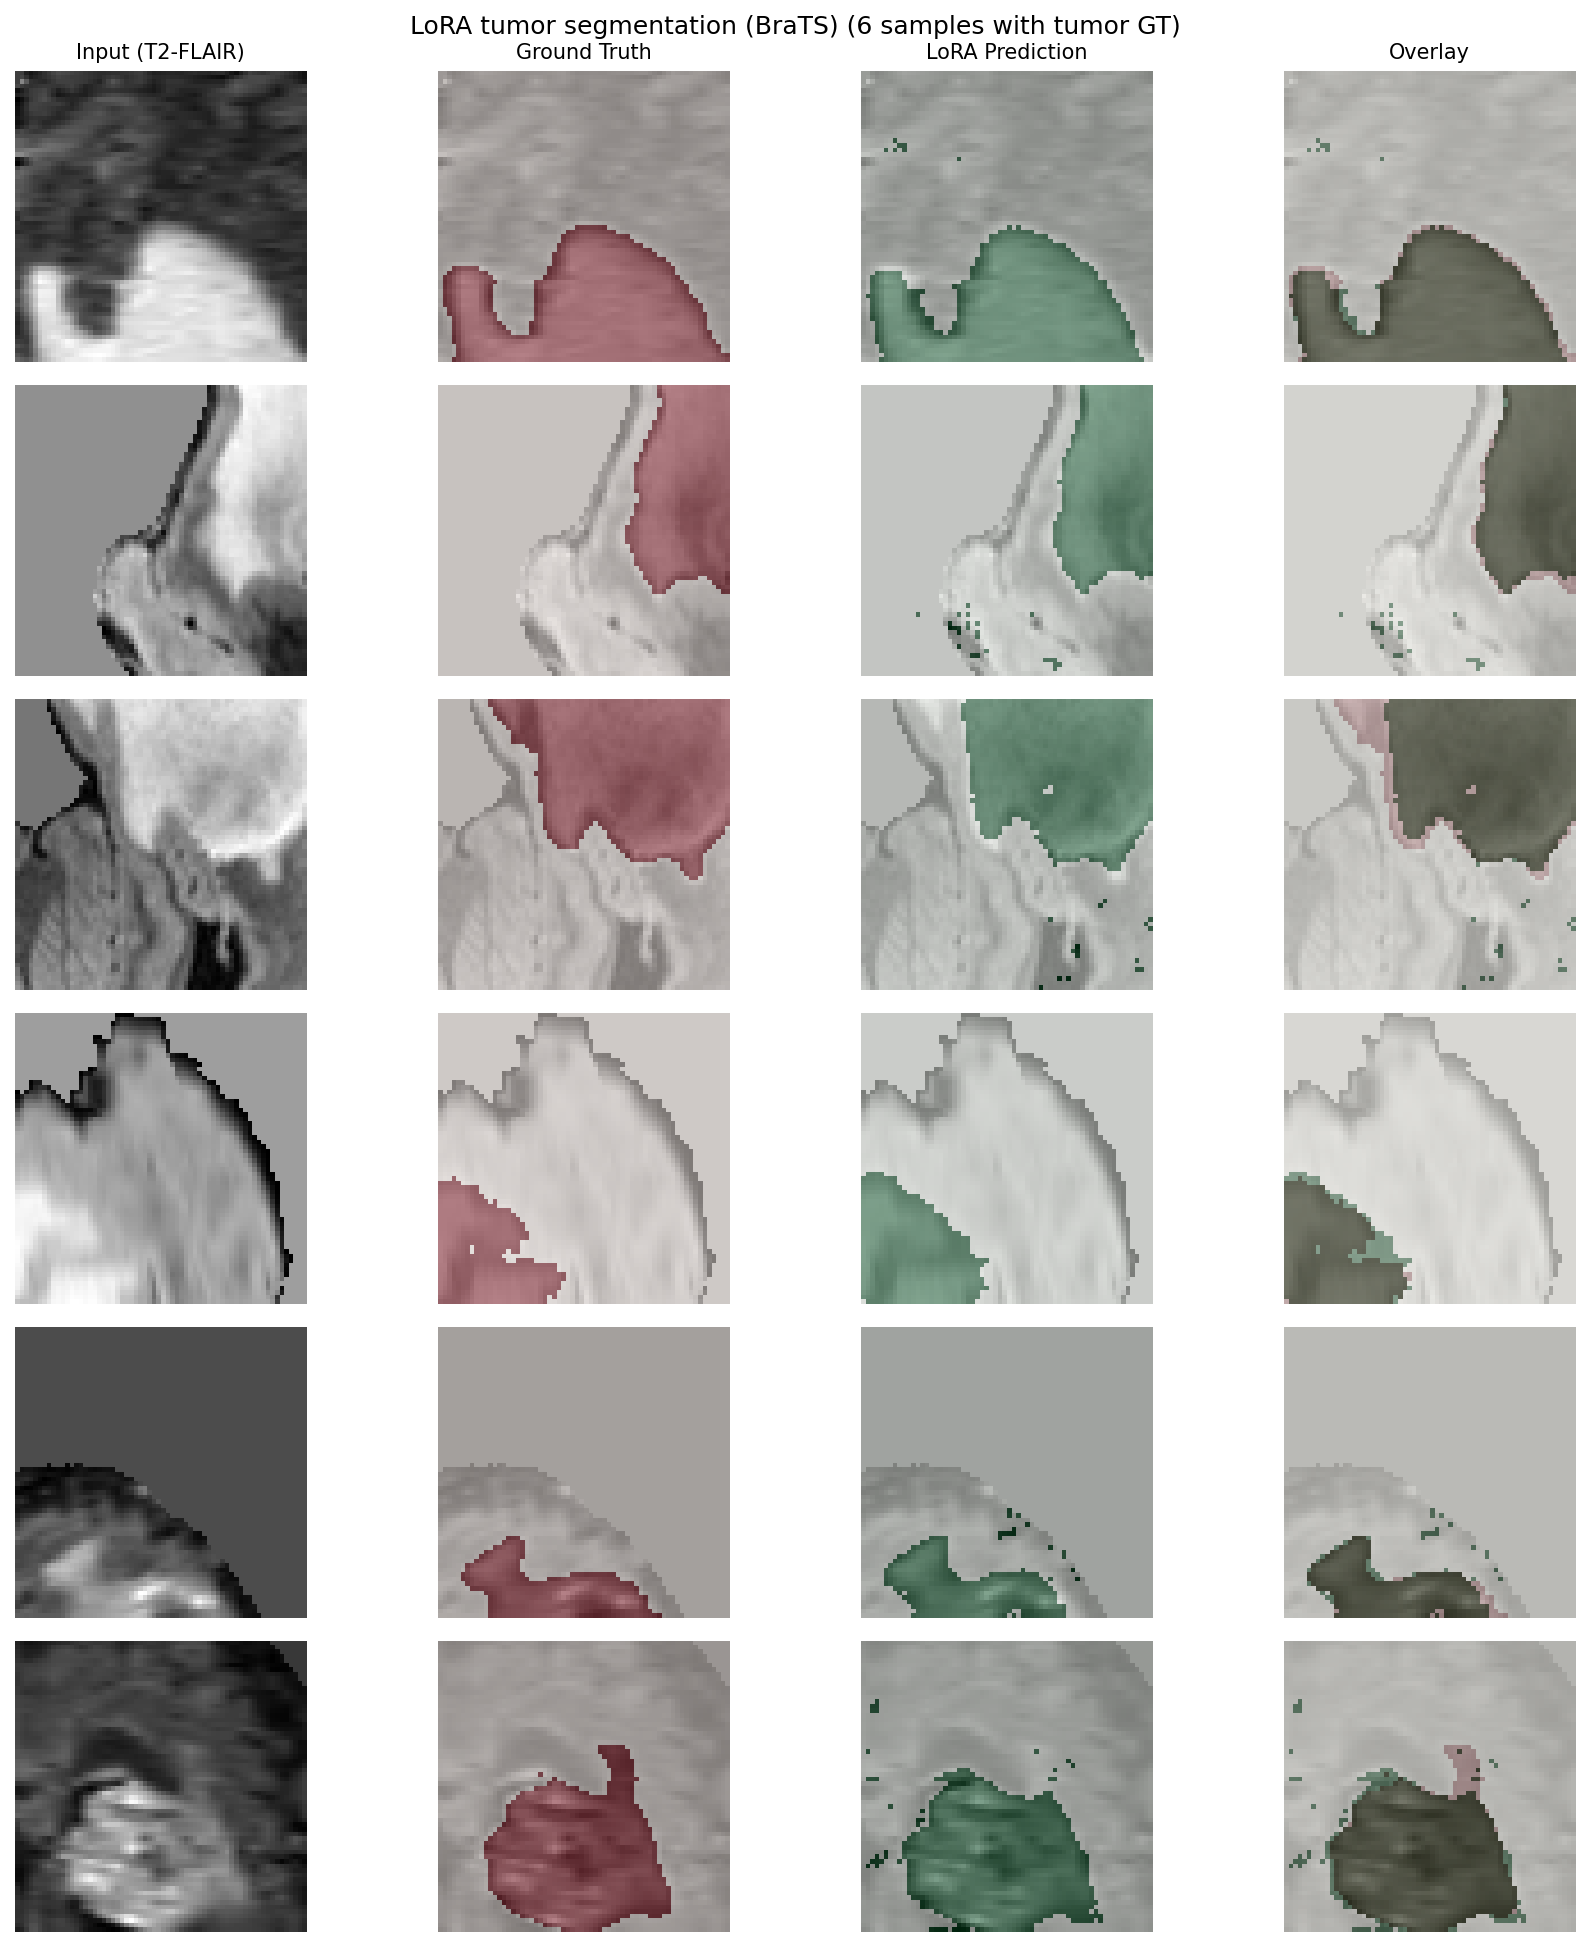
\includegraphics[width=0.95\textwidth]{figures/task2_seg_s42_stack6.png}
\caption{Task 1 tumor segmentation (BraTS): full six-sample stack. Input (T2-FLAIR), Ground Truth, LoRA prediction, overlay (red=GT, green=pred). Samples selected by highest slice-level Dice.}
\label{fig:app_seg_stack}
\end{figure}

\begin{figure}[t]
\centering
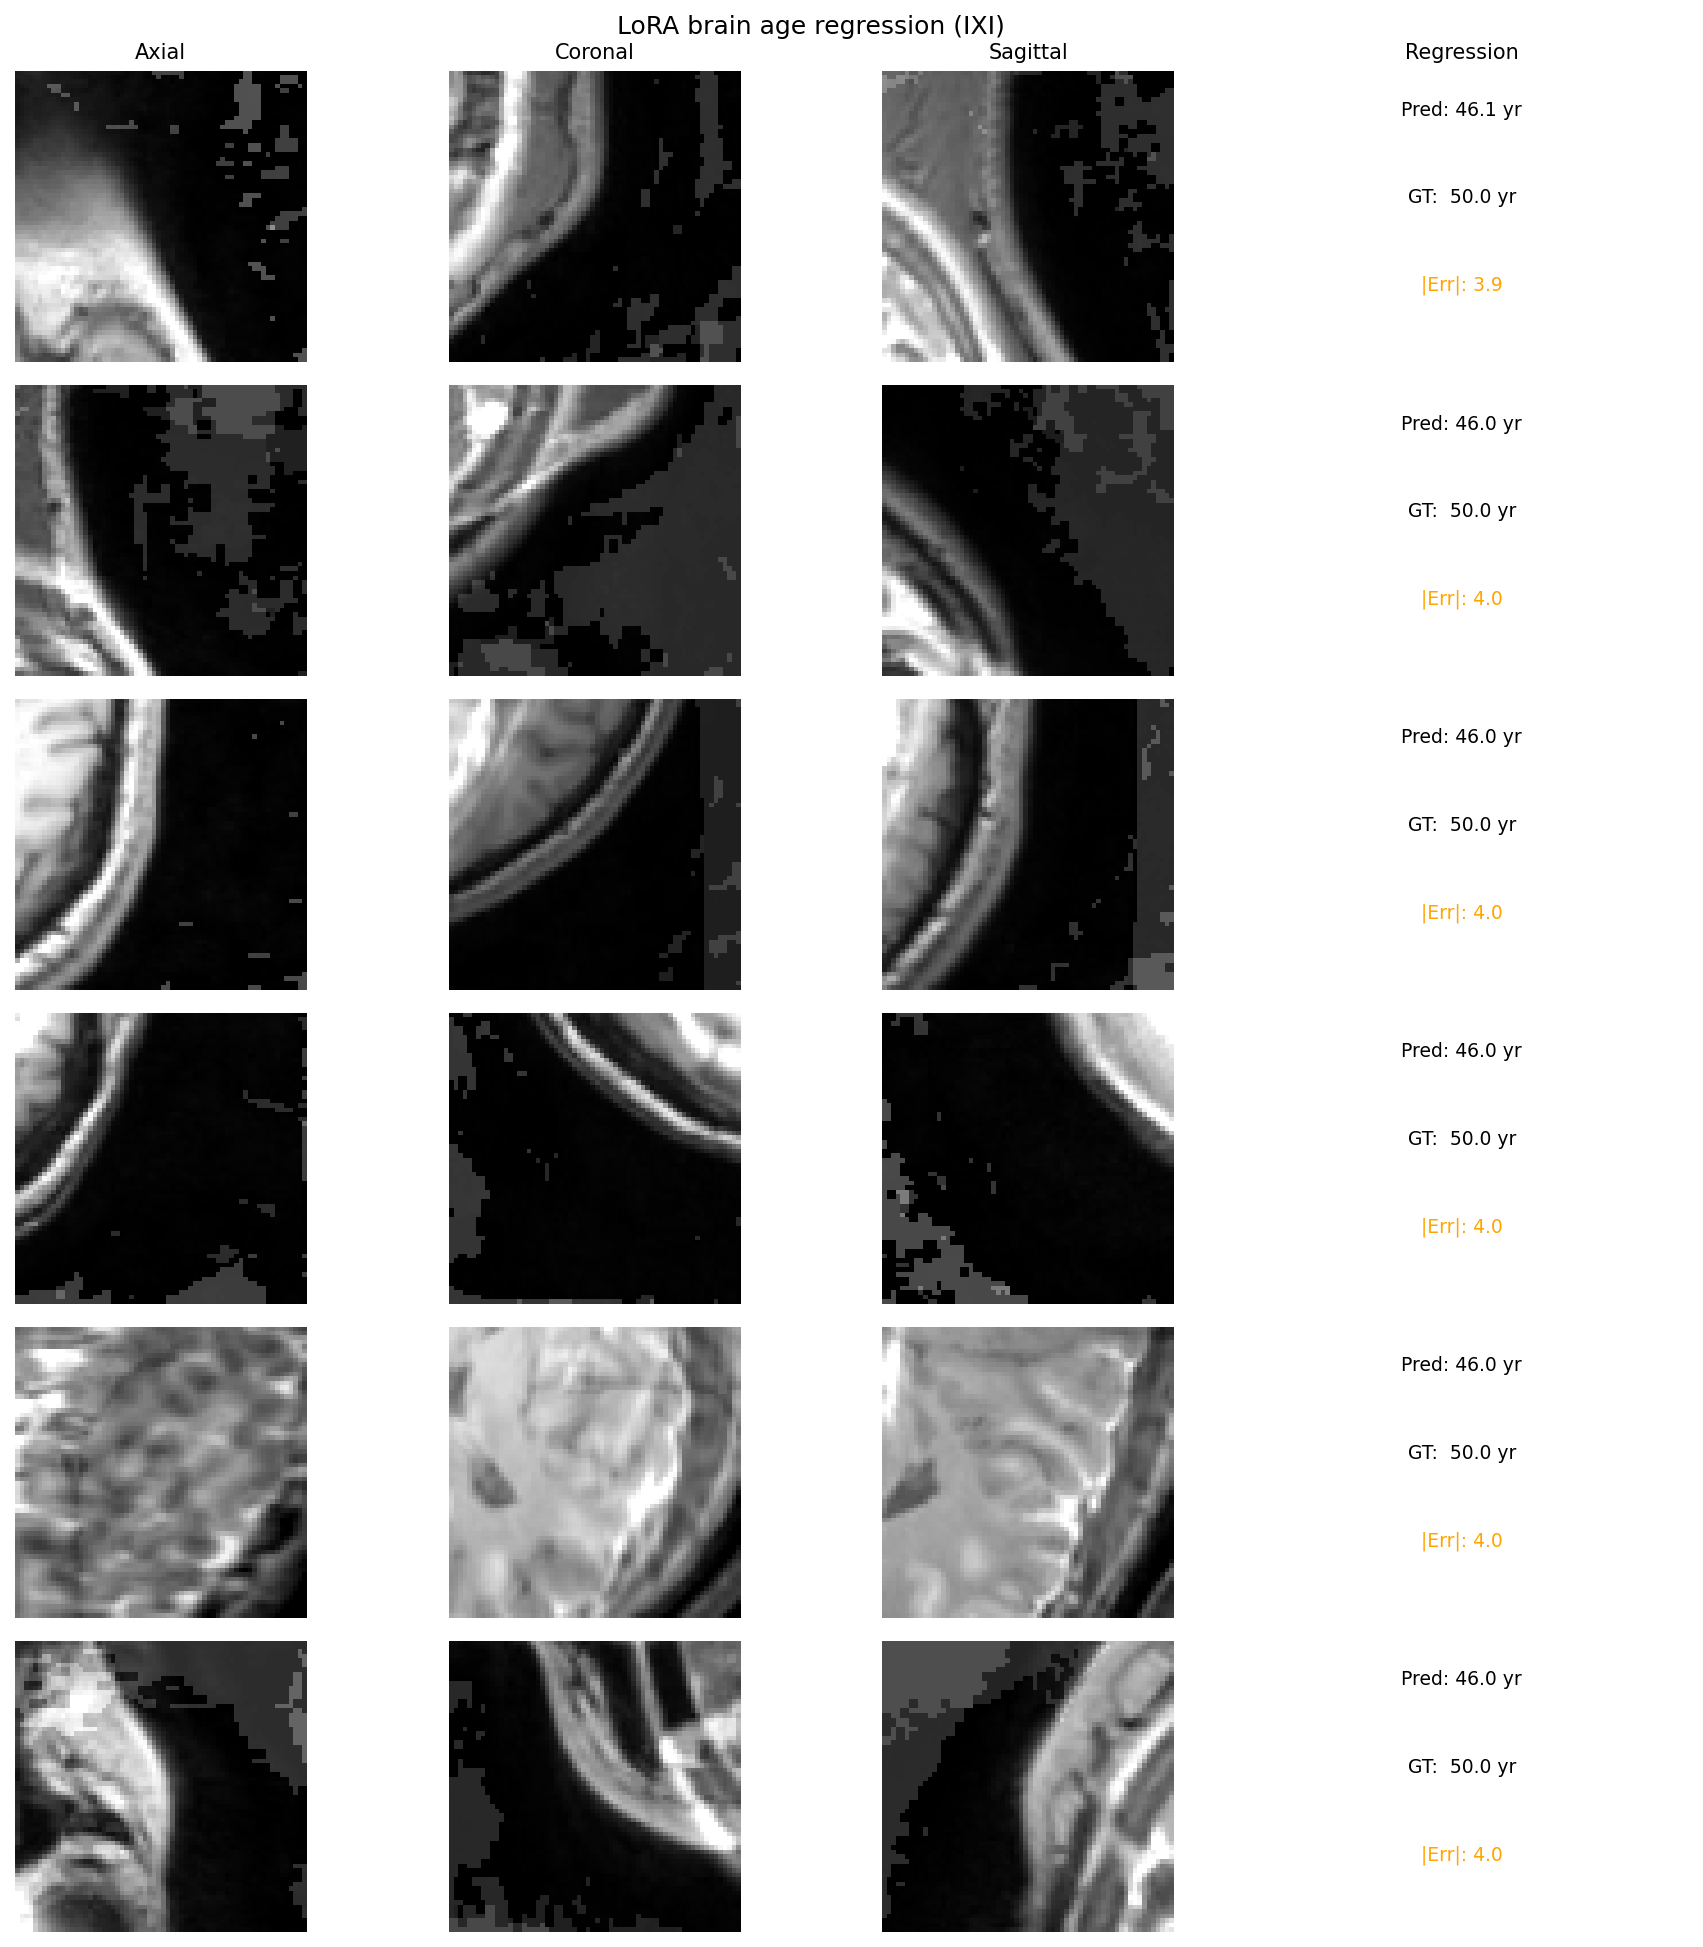
\includegraphics[width=0.95\textwidth]{figures/task3_age_s42_stack6.png}
\caption{Task 2 brain age regression (IXI): full six-sample stack. Orthogonal MRI views and regression results. Samples selected by lowest prediction error.}
\label{fig:app_age_stack}
\end{figure}

\subsection{Failure Case Examples}
\label{sec:appendix_failures}

\textbf{Under-segmentation (Task 1, BraTS):} In few-shot continual learning, LoRA can under-segment tumor boundaries, especially at lesion edges or in low-contrast regions. Figure~\ref{fig:app_seg_failure} shows six validation samples with the lowest slice-level Dice---LoRA predictions (green) miss portions of the ground-truth tumor (red) or produce fragmented masks.

\textbf{Age underestimation (Task 2, IXI):} As reported in the main text, Wilcoxon test indicates significant systematic underestimation ($p<0.001$). Figure~\ref{fig:app_age_failure} shows six samples with the largest prediction errors; the model tends to predict ages several years below the ground truth, consistent with the few-shot regime and IXI demographics.

\begin{figure}[t]
\centering
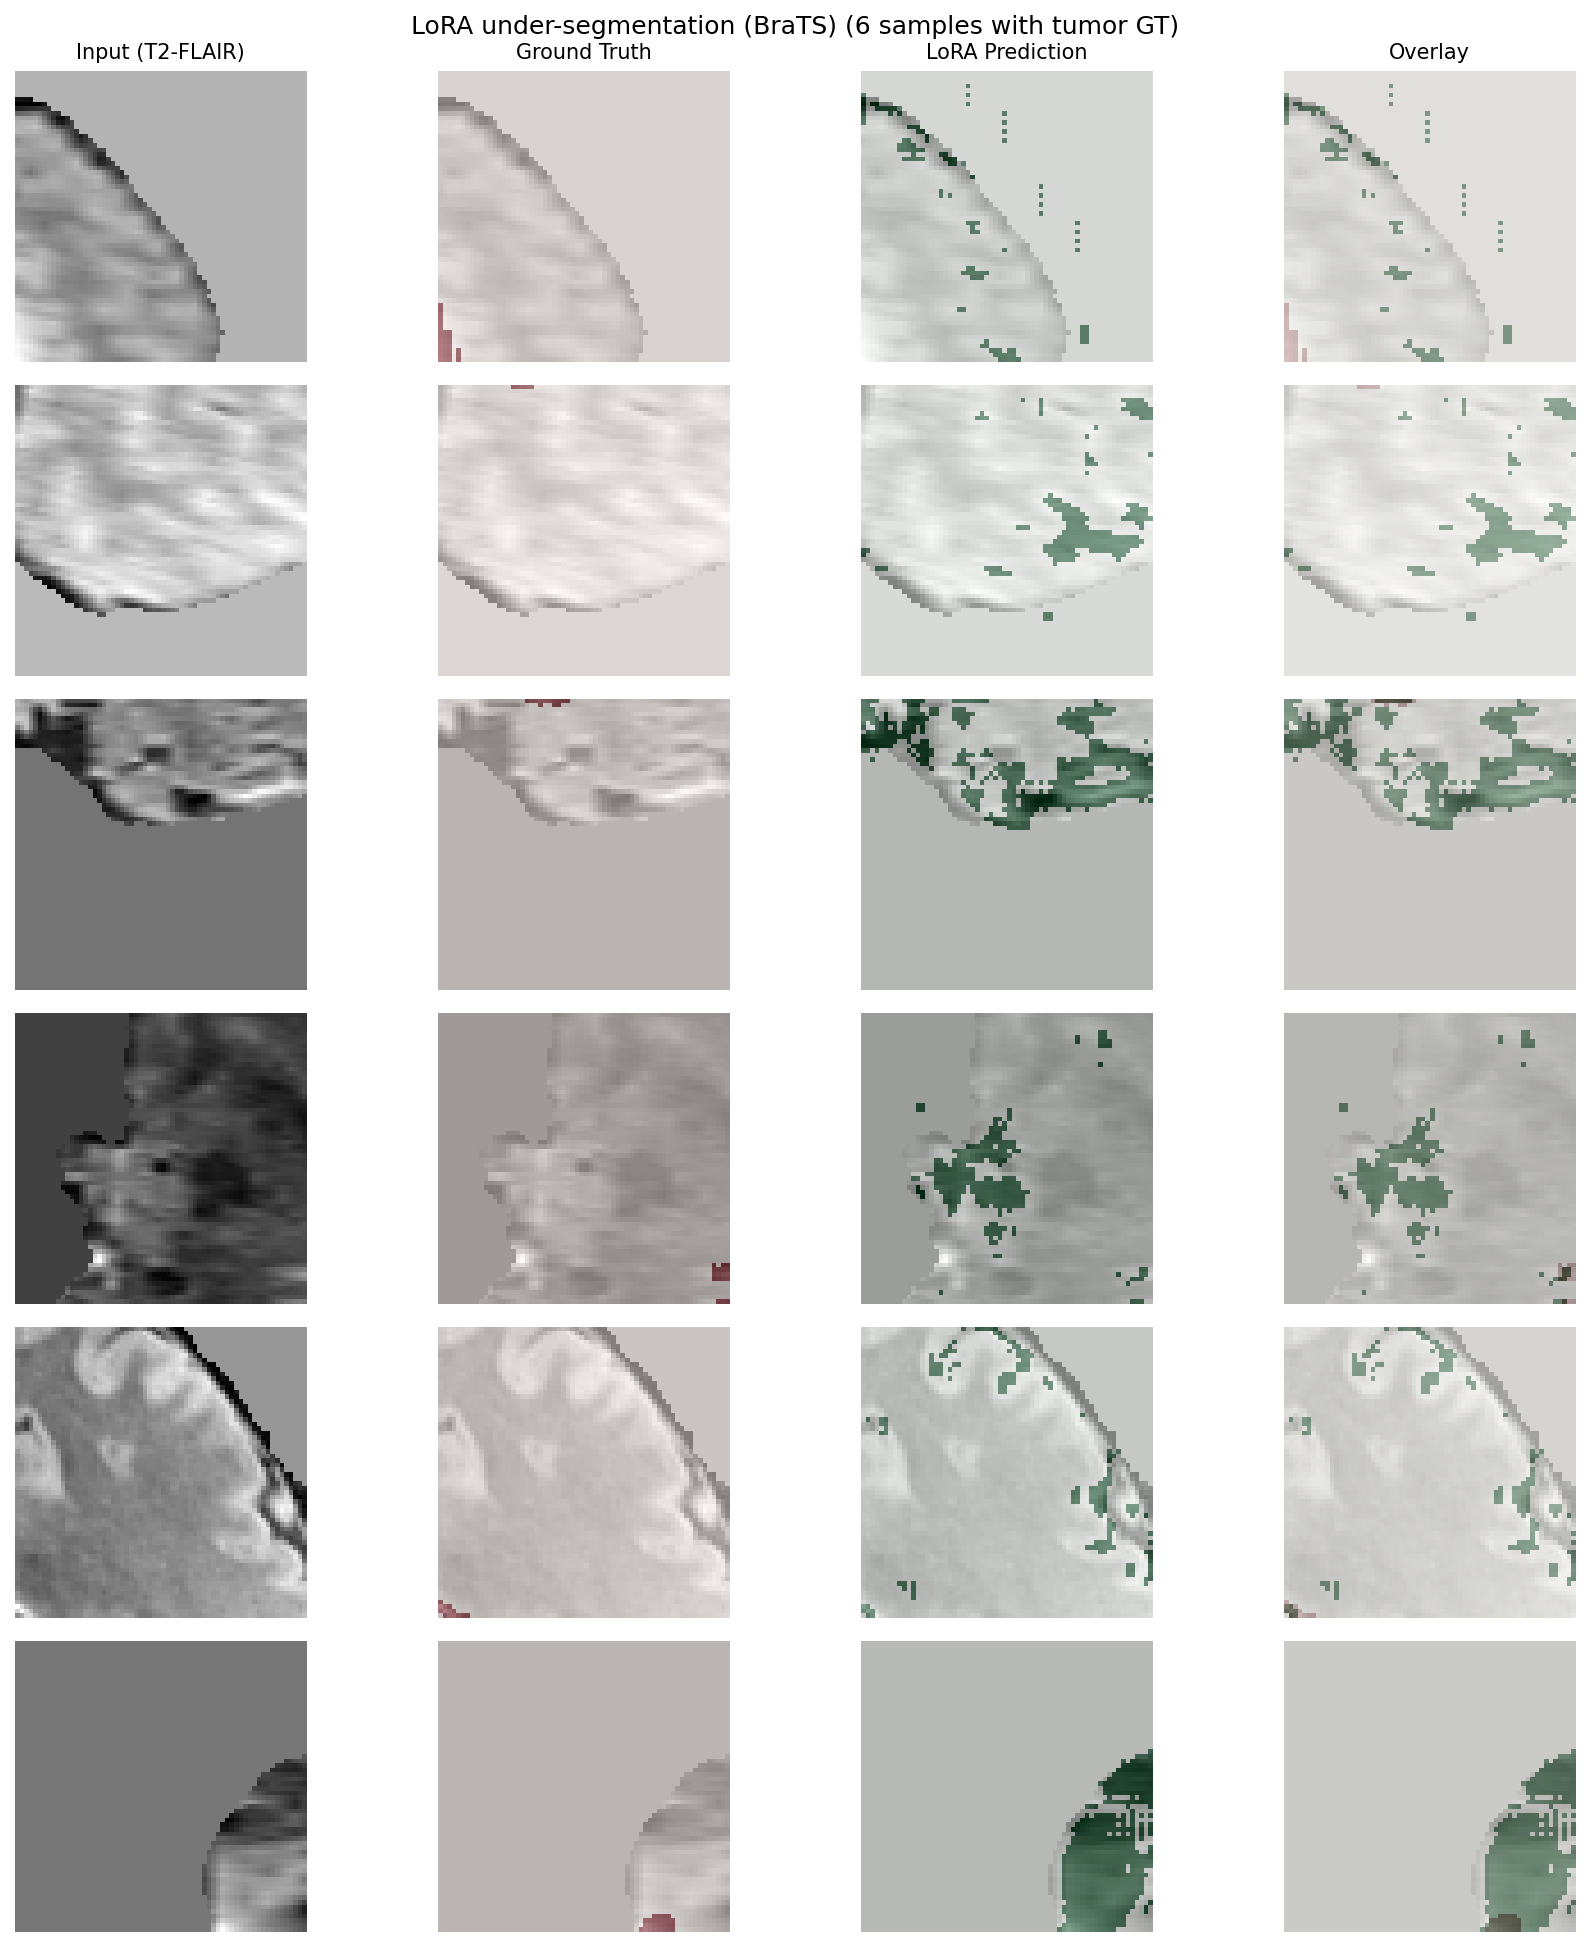
\includegraphics[width=0.95\textwidth]{figures/task2_seg_s42_stack6worst.png}
\caption{Task 1 failure cases: under-segmentation (BraTS). Six samples with lowest Dice. Red = ground truth; green = LoRA prediction.}
\label{fig:app_seg_failure}
\end{figure}

\begin{figure}[t]
\centering
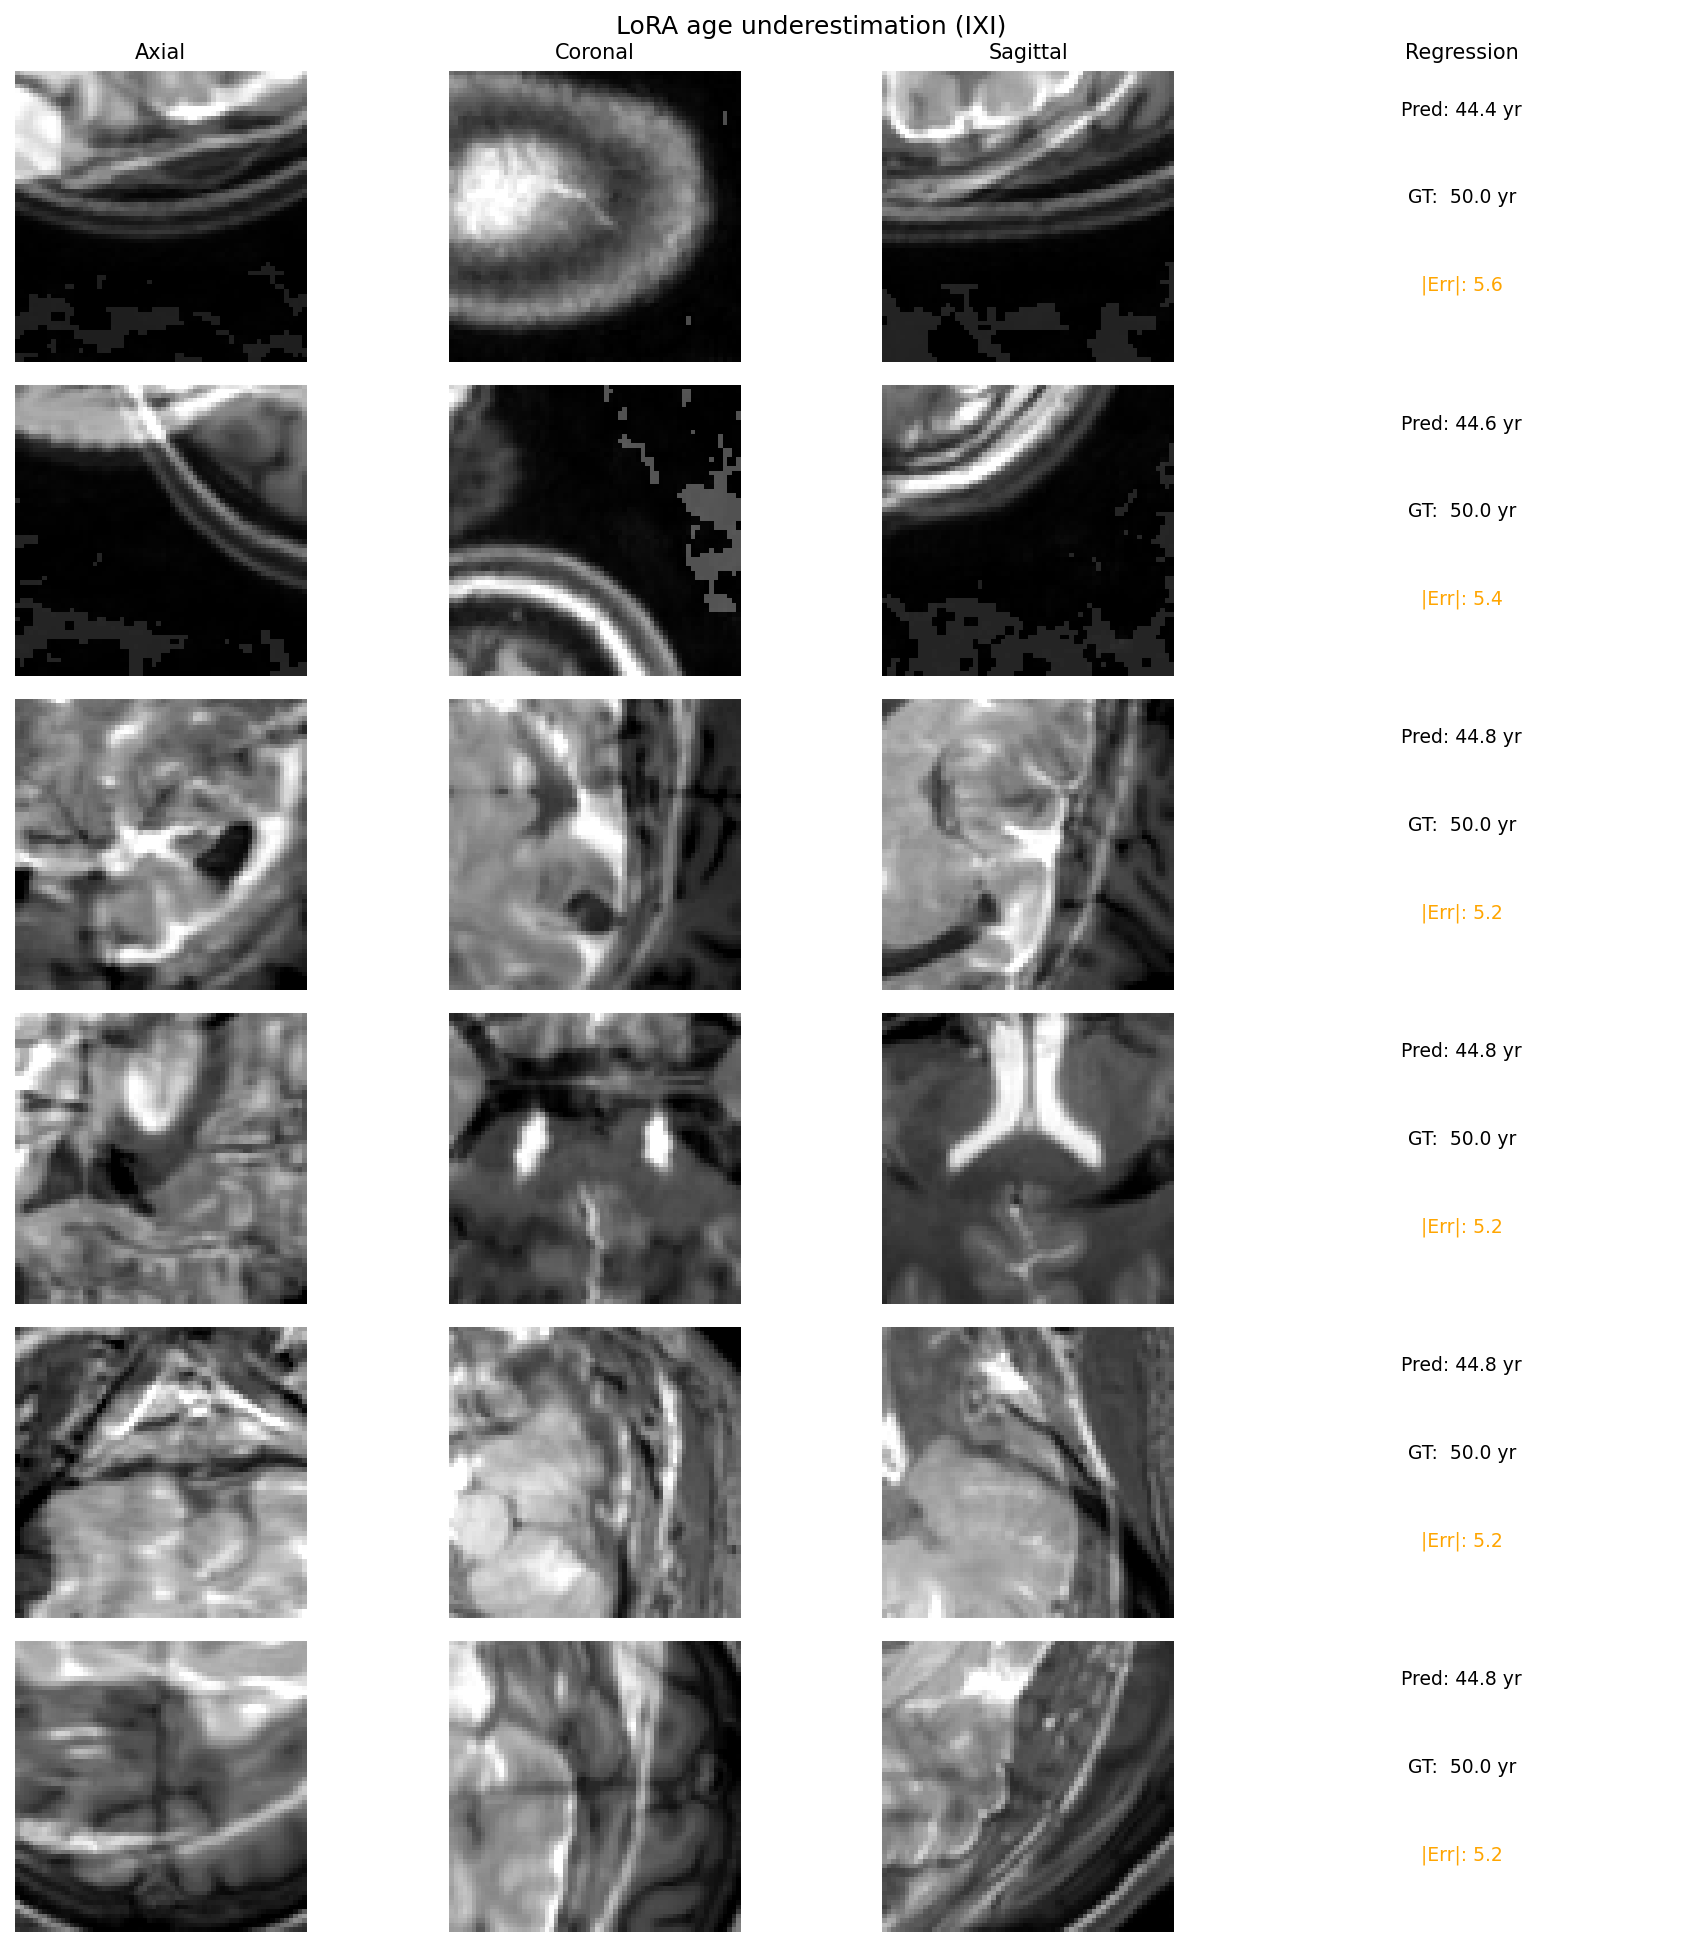
\includegraphics[width=0.95\textwidth]{figures/task3_age_s42_stack6worst.png}
\caption{Task 2 failure cases: age underestimation (IXI). Six samples with highest $|$predicted $-$ true$|$ error.}
\label{fig:app_age_failure}
\end{figure}
